% Stand-alone preview of the 6-page journal version of the Experimental Evaluation section (IEEEtran, compsoc, 10pt, two columns),
% numbered as Section 8 after Figures 1-7 and Tables 1-6 of the manuscript.
% Uses IEEEtran when installed; otherwise an article layout with the IEEE page geometry (7.16 in text width,
% 3.5 in columns, 10 pt Times), so that figure and table sizes match the manuscript.
\IfFileExists{IEEEtran.cls}{\documentclass[10pt,journal,compsoc]{IEEEtran}}{%
\documentclass[10pt,twocolumn]{article}
\usepackage[letterpaper,textwidth=7.16in,textheight=9.5in,columnsep=0.17in,top=0.7in]{geometry}
\usepackage{mathptmx}
\usepackage[font=footnotesize,labelsep=period]{caption}
\usepackage{titlesec}
\titleformat{\section}{\normalfont\large\scshape}{\thesection}{1em}{}
\titleformat{\subsection}{\normalfont\normalsize\itshape}{\thesubsection}{1em}{}
\renewcommand{\thetable}{\arabic{table}}}
\usepackage[nocompress]{cite}
\usepackage{graphicx}
\usepackage{booktabs}
\usepackage{multirow}
\usepackage{amsmath,amssymb}
\usepackage{url}
\usepackage{xcolor}
\newcommand{\pamcp}{PaMCP}
\graphicspath{{figures_r2/}}
\begin{document}
\setcounter{section}{7}
\setcounter{figure}{7}
\setcounter{table}{6}
\setcounter{equation}{7}
\setcounter{page}{13}
% ============================================================================================
% Section 8, journal version (6 pages): Experimental Evaluation of PaMCP.
% Figures: paper/figures_r2 (paper/make_eval_r2.py); tables: paper/tables_r2 and below.
% Every number is read from results/final/*.json and results/revision_2/*.json.
% ============================================================================================
\section{Experimental Evaluation}
\label{sec:ev}

\pamcp{} claims that discovery can be conditioned on the deployed model (RQ1), restricted to tools whose
safety-relevant behaviour is evidenced (RQ2), and returned as a small toolkit whose interfaces, effects and
flows are certified jointly before any call (RQ3), at a cost that scales and under registry change (RQ4). This
section tests each claim against the strongest baselines we could configure, labels every result by its evidence
class (\emph{measured} from the running system, \emph{observed} from executed servers, \emph{labelled} against
reference labels, \emph{simulated} under stated assumptions), and confirms the main comparisons with
pre-registered tests.

\subsection{Experimental Setup}
\label{sec:ev-setup}

\begin{table}[t]
\centering
\caption{Data and compared methods.}
\label{tab:ev-setup}
\scriptsize
\setlength{\tabcolsep}{2.5pt}
\begin{tabular}{@{}p{2.3cm}p{5.65cm}@{}}
\toprule
\multicolumn{2}{@{}l}{\emph{Data}} \\
Registry & 569 tools, 76 servers (LiveMCPTool \cite{mo2025livemcpbench} + MCPToolBench++ \cite{fan2025mcptoolbench}); 44 annotated \\
Multi-step tasks & 95 LiveMCPBench tasks (test); 60 development prompts \\
Single-tool requests & 60 development / 300 test (50 per category, 66 targets) \\
Calibration suite & 432 items: 6 operations, $n\in\{10,40,160,640\}$, en/fr, noise, context; 264 cal.\ / 168 test \\
Executed servers & 6 MCP reference servers, 37 registry tools \\
Synthetic & cloned and heterogeneous registries ($10^3$--$10^5$); 80 cover and 120 QoS instances \\
\midrule
\multicolumn{2}{@{}l}{\emph{Baselines (adapted to one registry, one encoder; tuned on the development split)}} \\
RAG-MCP \cite{gan2025ragmcp} & dense top-$k$ over the request \\
MCP-Zero \cite{fei2025mcpzero} & model-written requests, server routing \\
COLT \cite{qu2024colt} & collaborative graph of 450 training queries \\
ToolScope \cite{liu2026toolscope} & LLM-confirmed tool merging, subquery retrieval \\
CMTF \cite{suresh2026cmtf} & typed-state search, one tool per step \\
BM25, RRF, per-subtask & lexical, fused, one tool per analyst subgoal \\
\midrule
\multicolumn{2}{@{}l}{\emph{Ablations of \pamcp{}}} \\
G, P, S & gap (Alg.~1), eligibility (Sec.~5), set reasoning + certificate (Sec.~6), $2^3$ design \\
\pamcp{}-L & relevance-first ranking selected on the development split \\
\bottomrule
\end{tabular}
\end{table}

\begin{table}[t]
\centering
\caption{Parameters varied (default in bold).}
\label{tab:ev-params}
\scriptsize
\setlength{\tabcolsep}{2.5pt}
\begin{tabular}{@{}lp{4.3cm}@{}}
\toprule
Parameter & Values \\
\midrule
Profile threshold $\tau$ / risk target & 0.6, 0.75, \textbf{0.9} / 0.05, 0.10 \\
Forging servers $\delta$; false accepts $\varphi$ & 0--0.3 (5 seeds); 0--0.2, \textbf{0.05} \\
Probe coverage $\kappa$; trust $\ell_{\min}$ & 0.25--\textbf{1}; 0.2--0.95, \textbf{0.65} \\
Candidate budget $K$; size matching & 1, 5, \textbf{10}, 20, 40; equal $|K|$ \\
Poisoned descriptions; policies & 10\%, 30\%; least privilege, read-only \\
Registry size; pair relation & 569--$10^5$; eager, partitioned, \textbf{lazy} \\
Cost weights; utility floor $u_{\min}$ & 0, 0.25, \textbf{0.5}, 1; 0--0.9 \\
\bottomrule
\end{tabular}
\end{table}

Table~\ref{tab:ev-setup} lists the data and the methods and Table~\ref{tab:ev-params} the varied parameters.
Effects and types are scored against blind labels $J_B$ (Claude Opus) that are not used to simulate evidence;
the simulated verifier uses labels $J_A$ (Claude Sonnet), and we report the swapped direction and executed
servers to remove the dependency between the two. All LLM outputs were recorded once and are replayed. Every
method, including \pamcp{}, was configured on the development split only. Request-level metrics are resampled
with target tools as clusters and task-level metrics with tasks; paired tests are sign-flip permutation tests and
proportions use Wilson intervals (95\%). Two confirmatory families (F1--F7, H1--H5) were fixed before the data
they test and are Holm-corrected. Code, records, manifests and a notebook that re-runs every experiment on a
CPU are public.\footnote{\url{https://github.com/msellamiTN/taas-provenance-discovery}, branch
\texttt{research/pamcp-final-evaluation}; guide in \texttt{docs/REPRODUCIBILITY.md}.}

\subsection{RQ1: Model-Conditioned Representation}
\label{sec:ev-rq1}

\emph{Question.} Does a measured profile $\rho_{\mathrm{LLM}}$ decide reliably which operations the deployed model
keeps, and does the gap respond to the model and the input? \emph{Baselines:} the model's own
self-assessment and the earlier 64-item profile. \emph{Protocol:} three models answer the calibration suite by
reading only, after stating per cell their probability of success; $\tau$ is chosen on the calibration split for
a risk target and evaluated on held-out items (measured).

\begin{table}[t]
\centering
\caption{Model-profile calibration: accuracy (Wilson 95\% CI), self-assessment calibration, and the held-out
behaviour of the threshold $\tau$ chosen for a 5\% risk target (measured profile) versus the 64-item profile at
$\tau=0.9$. Cov.: share of operations kept native; FNR: false-native rate (errors among them).}
\label{tab:ev-calibration}
\scriptsize
\setlength{\tabcolsep}{2.2pt}
\begin{tabular}{@{}lrcrrrrrrrr@{}}
\toprule
 & & & & \multicolumn{2}{c}{Self-assess.} & \multicolumn{3}{c}{Measured, risk 5\%} & \multicolumn{2}{c}{64-item} \\
\cmidrule(lr){5-6}\cmidrule(lr){7-9}\cmidrule(l){10-11}
Model & $n$ & Accuracy (\%) & $n{=}640$ & ECE & Brier & $\tau$ & Cov. & FNR & Cov. & FNR \\
\midrule
Haiku & 432 & 86.1 [82.5, 89.1] & 67 & 0.39 & 0.30 & 0.21 & 83 & 3.6 & 21 & 0.0 \\
Sonnet & 432 & 91.4 [88.4, 93.7] & 62 & 0.20 & 0.11 & 0.42 & 90 & 3.3 & 26 & 4.5 \\
Opus & 387 & 100.0 [99.0, 100.0] & 100 & 0.38 & 0.20 & 0.90 & 100 & 0.0 & -- & -- \\
\bottomrule
\end{tabular}
\end{table}


\begin{figure*}[t]
\centering
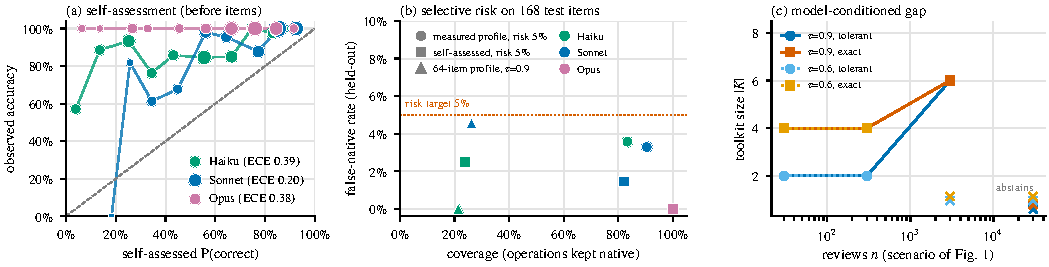
\includegraphics[width=\textwidth]{fig_rq1_profile}
\caption{RQ1. (a) Reliability of the models' self-assessment. (b) Held-out coverage and false-native rate of
the measured profile against the two baselines. (c) Toolkit size of the review scenario against the input size
(crosses: abstentions).}
\label{fig:ev-profile}
\end{figure*}

\emph{Results.} Capability boundaries differ by model and operation (Table~\ref{tab:ev-calibration}): Haiku fails
counting from $n=40$, Sonnet loses joins as they grow, and both fail approximate sums over 640 values; Opus answers
all 387 items it was given. With the measured profile and a 5\% risk target, the held-out false-native rate stays
within the target for every model (3.6\%, 3.3\%, 0.0\%) while 83--100\% of the operations remain with the model
(Fig.~\ref{fig:ev-profile}b). Both baselines fail: self-assessment is miscalibrated for every model (ECE
0.20--0.39, all underconfident; Fig.~\ref{fig:ev-profile}a), and the 64-item profile keeps only 21--26\% of the
operations native, sending most correctly performed work to tools. The gap behaves as designed
(Fig.~\ref{fig:ev-profile}c): two tools suffice for 30 or 300 reviews, six for 3,000, and the engine abstains
rather than return an unsupported toolkit at 30,000; without gap analysis it abstains in every setting. On the
test tasks the profile overrules 9.4\% of the analyst's claims that an operation is native. \emph{Answer:} a
measured, risk-targeted profile makes model conditioning reliable; neither self-assessment nor a small profile
can replace it.

\subsection{RQ2: Trust under Missing, Forged and Imperfect Evidence}
\label{sec:ev-rq2}

\emph{Question.} Does provenance-sound eligibility (P) keep unsafe tools away from the model, and at what cost?
\emph{Baselines:} no filter, MCP's default (annotations displayed, not enforced), annotations as a closed world,
and lexical cues, each combined with \pamcp{}'s retrieval and with MCP-Zero. \emph{Protocol:} read-only policy
over 273 requests with read-only gold tools; Exp@5 is the share whose top five contain a tool that is not read-only
under $J_B$, Util@5 the share containing a gold tool; forgery and verifier errors are simulated.

\begin{table}[t]
\centering
\caption{Encodings of a read-only policy over 273 requests with read-only gold tools: eligible share of the
registry, unsafe tools admitted (of 120, $J_B$), exposure and utility of the top five for \pamcp{}'s retrieval
stage and MCP-Zero, and exposure when 20\% of the servers forge and launder their metadata (verifier
false-accept rate 5\%, mean of five seeds).}
\label{tab:ev-encodings}
\scriptsize
\setlength{\tabcolsep}{2.2pt}
\begin{tabular}{@{}lrrrrrrr@{}}
\toprule
 & & & \multicolumn{2}{c}{\pamcp{} retr.} & \multicolumn{2}{c}{MCP-Zero} & $\delta{=}0.2$ \\
\cmidrule(lr){4-5}\cmidrule(lr){6-7}\cmidrule(l){8-8}
Encoding & Elig. & Unsafe & Exp@5 & Util@5 & Exp@5 & Util@5 & Exp@5 \\
\midrule
no filter & 100.0 & 120 & 42.5 & 49.8 & 26.4 & 76.6 & 43.7 \\
MCP default (display only) & 100.0 & 120 & 42.5 & 49.8 & 26.4 & 76.6 & 43.7 \\
closed-world annotations & 7.7 & 1 & 31.5 & 0.4 & 0.0 & 0.4 & 58.7 \\
lexical cues & 67.8 & 21 & 9.9 & 41.0 & 12.5 & 65.6 & 8.8 \\
verified evidence (P) & 77.0 & 0 & 0.0 & 46.2 & 0.0 & 72.2 & 5.5 \\
observed + lexical fallback & 77.0 & 0 & 0.0 & 46.2 & 0.0 & 72.2 & 5.5 \\
attested only & 26.4 & 0 & 0.0 & 16.5 & 0.0 & 18.3 & 5.8 \\
\bottomrule
\end{tabular}
\end{table}


\begin{figure*}[t]
\centering
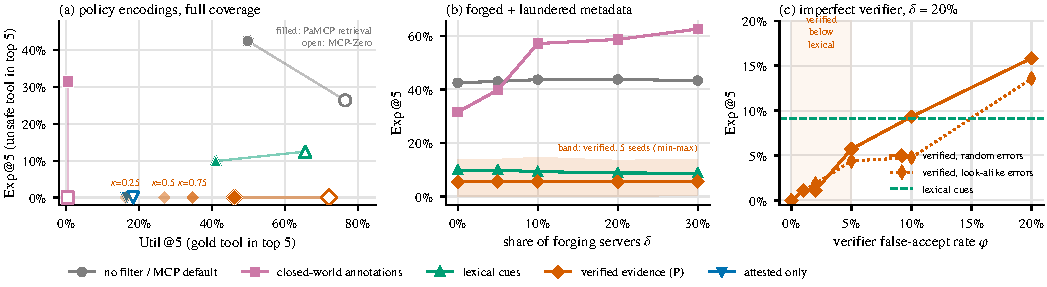
\includegraphics[width=\textwidth]{fig_rq2_exposure}
\caption{RQ2. (a) Exposure against utility per policy encoding (filled: \pamcp{} retrieval, open: MCP-Zero) and
under lower probe coverage $\kappa$. (b) Exposure as a share $\delta$ of servers forges annotations and launders
descriptions (band: five seeds). (c) Exposure against the verifier's false-accept rate.}
\label{fig:ev-exposure}
\end{figure*}

\emph{Results.} Every baseline encoding exposes unsafe tools (Table~\ref{tab:ev-encodings}): 42.5\% of the
requests without a filter or under MCP's default, 31.5\% with annotations as a closed world (whose utility falls to
0.4\%), and 9.9\% with lexical cues. Verified evidence admits none of the 120 unsafe tools, keeps 77\% of the
registry eligible and costs 3.6 utility points (4.4 for MCP-Zero); the difference to lexical cues is confirmatory
(F4: $-9.9$ points, $p_{\mathrm{Holm}}<0.001$). Under forgery the closed-world reading collapses (31.5\% to 62.6\%
exposure at $\delta=0.3$) while verified evidence stays at 5.4--5.6\% for every $\delta$ with a 5\% false-accept
rate (Fig.~\ref{fig:ev-exposure}b), and it remains below lexical cues up to $\varphi=5\%$ (10\% for look-alike
errors; Fig.~\ref{fig:ev-exposure}c). Three checks remove the dependency on how the labels were built. With the
verifier simulated from $J_B$ and scored on $J_A$, exposure is 2.3--3.9\% across \pamcp{}, RAG-MCP, MCP-Zero and
ToolScope, a quarter to two fifths of the exposure left by lexical cues. Executing the six MCP reference servers under system-call
tracing (observed; Fig.~\ref{fig:ev-observed}), both labellings agree with all 30 completed calls: none of the 13 tools observed to change
state is labelled read-only (Wilson upper bound 22.8\%). And every one of the 37 surviving definitions changed
since the benchmark snapshot, so evidence not bound to $h(t)$, as \pamcp{} binds it, would have been stale.
\emph{Answer:} eligibility based on verified, hash-bound evidence removes the exposure that published metadata
leaves, degrades in proportion to verifier error, and does not depend on the reference labels.

\begin{figure*}[t]
\centering
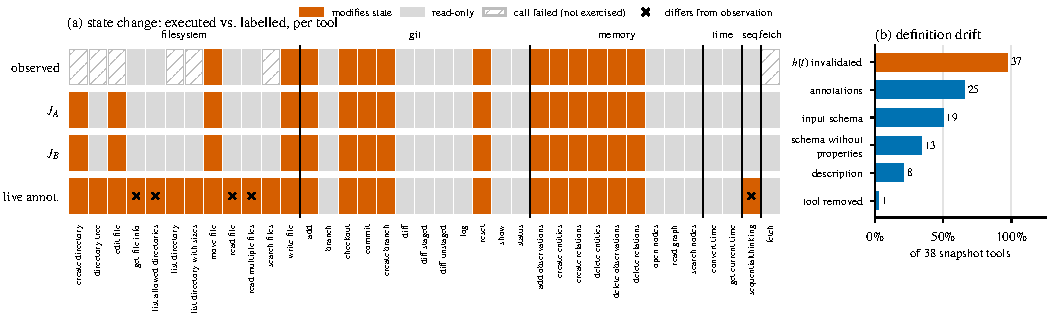
\includegraphics[width=\textwidth]{fig_rq2_observed}
\caption{RQ2, executed reference servers (observed). (a) Per registry tool: state change observed under tracing
against the two labellings and the servers' current annotations. (b) Changes of the live definitions since the
benchmark snapshot; every change alters $h(t)$ and invalidates bound evidence.}
\label{fig:ev-observed}
\end{figure*}

\subsection{RQ3: Composition and Certification}
\label{sec:ev-rq3}

\emph{Question.} Does set-level reasoning return smaller toolkits that are jointly feasible more often than
retrieval? \emph{Baselines:} RAG-MCP, COLT, ToolScope (top five), MCP-Zero, CMTF and per-subtask retrieval, each
also restricted to eligible tools. \emph{Protocol:} 94 test tasks; group recall against benchmark gold
(measured); joint feasibility decided by two evaluators written independently of the certificate, a coarse one and
a strict one that also checks domains, cardinality, schema-required inputs and egress of private data (labelled).
On ten hand-built cases with known answers the strict evaluator decides 7 correctly, the coarse one 2.

\begin{table}[t]
\centering
\caption{Toolkits on the 94 LiveMCPBench test tasks: size, manifest tokens, group recall (task bootstrap 95\%
CI), share of toolkits jointly feasible for the coarse and the strict independent evaluator (least-privilege
policies), and abstentions. Baselines restricted to eligible tools unless marked published.}
\label{tab:ev-sets}
\scriptsize
\setlength{\tabcolsep}{2.1pt}
\begin{tabular}{@{}lrrlrrr@{}}
\toprule
 & & & & \multicolumn{2}{c}{Joint feas. (\%)} & \\
\cmidrule(lr){5-6}
Method & $|K|$ & Tok. & Group recall [CI] & coarse & strict & Abst. \\
\midrule
\pamcp{} ($K{=}10$) & 1.46 & 198 & 0.174 [0.12, 0.23] & 67.0 & 27.7 & 7.4 \\
\pamcp{}-L & 1.22 & 146 & 0.161 & 54.7 & 15.8 & 9.5 \\
\pamcp{} NoCert & -- & -- & -- & 59.6 & 13.8 & 0.0 \\
Per-subtask (elig.) & 2.59 & 346 & 0.249 [0.19, 0.32] & 62.8 & 8.5 & -- \\
RAG-MCP@5 (elig.) & 5.00 & 1244 & 0.293 [0.22, 0.37] & 60.6 & 5.3 & -- \\
COLT@5 (elig.) & 5.00 & 1094 & 0.295 [0.23, 0.37] & 59.6 & 8.5 & -- \\
ToolScope@5 (elig.) & 5.20 & 976 & 0.361 [0.29, 0.44] & 73.4 & 11.7 & -- \\
MCP-Zero (elig.) & 1.76 & 250 & 0.227 [0.17, 0.29] & 57.4 & 11.7 & -- \\
CMTF (elig.) & 0.64 & 105 & 0.072 [0.04, 0.11] & 25.5 & 14.9 & -- \\
RAG-MCP@5 (published) & 5.00 & 1244 & 0.293 [0.22, 0.37] & 48.9 & 5.3 & -- \\
\bottomrule
\end{tabular}
\end{table}


\begin{figure*}[t]
\centering
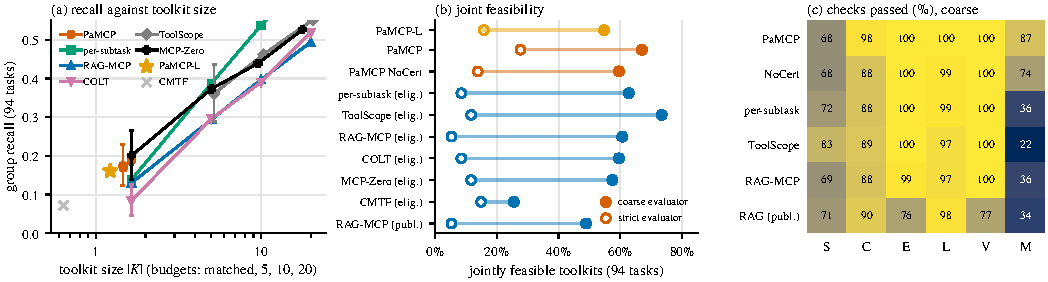
\includegraphics[width=\textwidth]{fig_rq3_sets}
\caption{RQ3. (a) Group recall against toolkit size for candidate budgets. (b) Jointly feasible toolkits under the
coarse and the strict evaluator. (c) Checks passed: goals served (S), inputs obtainable (C), effects (E), flows
(L), evidence (V), minimality (M).}
\label{fig:ev-sets}
\end{figure*}

\emph{Results.} \pamcp{} returns the smallest toolkits apart from CMTF, 1.46 tools and 198 tokens against 5 tools
and 976--1,244 tokens for the top-five retrievers (Table~\ref{tab:ev-sets}), and it certifies 92.6\% of the tasks,
abstaining with a counterexample on the rest. Under the strict evaluator its toolkits are jointly feasible in
27.7\% of the tasks, 1.9 to 5.2 times as often as every baseline restricted to eligible tools (5.3--14.9\%) and twice as
often as without certification (13.8\%; Fig.~\ref{fig:ev-sets}b). Certification acts through obtainable inputs and
minimality (C 88\% to 98\%, M 74\% to 87\%, against 22--36\% for the top-five retrievers;
Fig.~\ref{fig:ev-sets}c). At equal size \pamcp{} reaches more gold steps than RAG-MCP, per-subtask retrieval and
COLT (0.189 against 0.130, 0.138 and 0.084; F2 not significant after correction), whereas retrievers that expose
three to four times more tools reach more (0.249--0.361; non-inferiority to per-subtask retrieval, F1, not shown):
\pamcp{} trades breadth for certified compactness.

\begin{table}[t]
\centering
\caption{Single-tool retrieval on the 300 test requests with configurations selected on the development split:
Hit@1 over the 81 MCPToolBench++ tools and, with target-tool clustered 95\% CI, over the 569-tool registry, and
the other metrics over 569 tools.}
\label{tab:ev-retrieval}
\scriptsize
\setlength{\tabcolsep}{2.4pt}
\begin{tabular}{@{}lrrrrrr@{}}
\toprule
 & 81 tools & \multicolumn{5}{c}{569 tools} \\
\cmidrule(lr){2-2}\cmidrule(l){3-7}
Method & Hit@1 & Hit@1 [CI] & Hit@3 & Hit@5 & MRR & nDCG \\
\midrule
BM25 & 52.7 & 41.0 [26, 60] & 57.3 & 63.7 & 0.503 & 0.543 \\
RAG-MCP (dense) & 49.7 & 37.3 [22, 56] & 50.0 & 54.3 & 0.451 & 0.492 \\
RRF fusion & 54.3 & 38.7 [23, 57] & 54.7 & 61.3 & 0.481 & 0.525 \\
MCP-Zero & 68.0 & 66.7 [49, 80] & 80.0 & 85.7 & 0.743 & 0.775 \\
COLT & 49.7 & 37.3 [22, 56] & 50.0 & 54.3 & 0.451 & 0.492 \\
ToolScope & 53.0 & 41.0 [26, 60] & 58.3 & 63.7 & 0.504 & 0.543 \\
CMTF & 58.7 & 32.7 [19, 49] & 47.0 & 54.7 & 0.428 & 0.488 \\
PaMCP (Eq. 5) & 61.0 & 29.7 [16, 47] & 45.7 & 53.7 & 0.400 & 0.461 \\
PaMCP-L & 72.0 & 41.3 [25, 60] & 61.3 & 69.3 & 0.536 & 0.603 \\
PaMCP, oracle types (diag.) & 71.7 & 58.3 [38, 74] & 75.3 & 81.3 & 0.680 & 0.728 \\
\bottomrule
\end{tabular}
\end{table}


\emph{Boundary: single-tool retrieval.} Retrieval is not where \pamcp{} gains (Table~\ref{tab:ev-retrieval}).
Over 81 tools its relevance-first ranking is the most accurate (72.0\% Hit@1, MCP-Zero 68.0\%), but over the full
registry MCP-Zero leads (66.7\%), \pamcp{}-L ties tuned BM25 (41.3\% against 41.0\%; H1 n.s.) and the structural
ranking of Eq.~(5) falls to 29.7\% (F7 against \pamcp{}), because types agree with $J_B$ on 78.9\% of output kinds
but only 35.7\% of domains. With correct types the same ranking reaches 58.3\%, above every baseline except
MCP-Zero, which locates the limit in the typing rather than in the composition. \emph{Answer:} set-level reasoning
yields the most compact and most often jointly feasible toolkits; finding more tools requires better typing or a
larger budget.

\subsection{RQ2/RQ3: Security and Contribution of the Mechanisms}
\label{sec:ev-sec}

\emph{Question.} Does the exposed toolkit limit what an injected instruction could achieve, and which mechanism is
responsible? \emph{Protocol:} for 155 tasks and each attack class outside the task's needs, an attack is reachable
if the toolkit can realise it under $J_B$ (labelled, offline); poisoning places a canary in the description, name or
argument keys of 10--30\% of the tools and scans what each method shows the model; the mechanisms are varied in a
$2^3$ design with Shapley attribution.

\begin{figure*}[t]
\centering
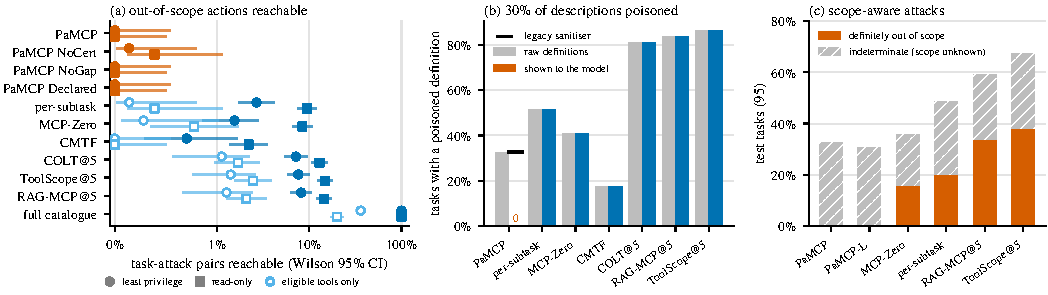
\includegraphics[width=\textwidth]{fig_sec_injection}
\caption{Security. (a) Task--attack pairs reachable for each method, as published (filled) and restricted to
eligible tools (open), under two policies (Wilson 95\% CI). (b) Tasks whose definitions carry an injected
instruction, raw against shown to the model. (c) Test tasks with an attack definitely out of scope or of
undecidable scope.}
\label{fig:ev-injection}
\end{figure*}

\emph{Results.} No out-of-scope action is reachable through \pamcp{}'s toolkits: 0 of 712 task--attack pairs under
least privilege and 0 of 775 under a read-only policy, against 0.7--8.1\% and 8.4--14.7\% for the published
baselines (Fig.~\ref{fig:ev-injection}a; F5, $p_{\mathrm{Holm}}<0.001$). Counting only attacks that are definitely
out of scope, no \pamcp{} toolkit admits one, against 15.8\% of the tasks for MCP-Zero, 20.0\% for per-subtask
retrieval, 33.7\% for RAG-MCP and 37.9\% for ToolScope (H5: $-20.0$ points, 95\% CI $[-28.4,-12.6]$,
$p_{\mathrm{Holm}}<0.001$); 32.6\% admit an attack whose scope the labels cannot decide. With 30\% of the
descriptions poisoned, the aliased manifest never shows an injected instruction, whereas the definitions exposed
by the baselines carry one in 17.4--86.2\% of the tasks (Fig.~\ref{fig:ev-injection}b); 55.5\% of \pamcp{}'s
toolkits return remote content, but none of them also enables an out-of-scope action (3.2--22.6\% for the
baselines).

\begin{table}[t]
\centering
\caption{Mechanism ablation on 155 tasks under least-privilege policies: the $2^3$ design over the gap (G),
provenance-sound eligibility (P) and set-level reasoning (S), and five components of the full configuration.
Reach: task--attack pairs whose out-of-scope action the toolkit can realise.}
\label{tab:ev-factorial}
\scriptsize
\setlength{\tabcolsep}{3pt}
\begin{tabular}{@{}cccrrrrr@{}}
\toprule
G & P & S & Recall & Tokens & Joint (\%) & Reach (\%) & Abst. (\%) \\
\midrule
-- & -- & -- & 0.270 & 297 & 53.5 & 1.1 & 0.0 \\
on & -- & -- & 0.239 & 208 & 55.5 & 0.4 & 0.0 \\
-- & on & -- & 0.295 & 316 & 58.1 & 0.1 & 0.0 \\
-- & -- & on & 0.223 & 221 & 52.9 & 0.1 & 16.1 \\
on & on & -- & 0.253 & 229 & 56.8 & 0.1 & 0.0 \\
on & -- & on & 0.230 & 189 & 54.8 & 0.0 & 6.5 \\
-- & on & on & 0.183 & 193 & 55.5 & 0.0 & 20.0 \\
on & on & on & 0.181 & 176 & 56.1 & 0.0 & 10.3 \\
\midrule
\multicolumn{3}{@{}l}{Full, no backward closure} & 0.181 & 173 & 53.5 & 0.0 & 12.3 \\
\multicolumn{3}{@{}l}{Full, flow along derivations} & 0.236 & 206 & 60.6 & 0.0 & 5.8 \\
\multicolumn{3}{@{}l}{Full, no relevance term} & 0.167 & 141 & 54.8 & 0.0 & 10.3 \\
\multicolumn{3}{@{}l}{Full, no utility floor} & 0.181 & 176 & 56.1 & 0.0 & 10.3 \\
\multicolumn{3}{@{}l}{Full, no refinement} & 0.179 & 175 & 55.5 & 0.0 & 11.0 \\
\bottomrule
\end{tabular}
\end{table}


The factorial design (Table~\ref{tab:ev-factorial}) shows that each mechanism contributes. Eligibility removes
most reachable actions, and with gap analysis and set reasoning reachability falls from 5.2\% of the tasks to none
(Shapley shares 23\%, 35\% and 42\% for G, P and S). Gap analysis and set reasoning shrink the context from 297 to
176 tokens (main effects $-56$ and $-67$ tokens, $p<0.001$), and the gap halves abstentions (10.3\% against
20.0\%). The price is recall (0.270 to 0.181, mainly through S); no mechanism changes the coarse joint
feasibility. \emph{Answer:} under the labelled threat model, \pamcp{}'s mechanisms jointly close the action and
metadata channels that retrieval baselines leave open.

\subsection{RQ3/RQ4: Efficiency, Optimality and Evolution}
\label{sec:ev-eff}

\emph{Question.} What does discovery cost, how close is the composition to the optimum, and does the engine keep
its guarantees under change? \emph{Baselines:} eager materialisation of the risk relation, the greedy regime and an
integer program (HiGHS) written independently of the engine, full rebuilds and cache flushes, and cold discovery
without experience reuse.

\begin{figure*}[t]
\centering
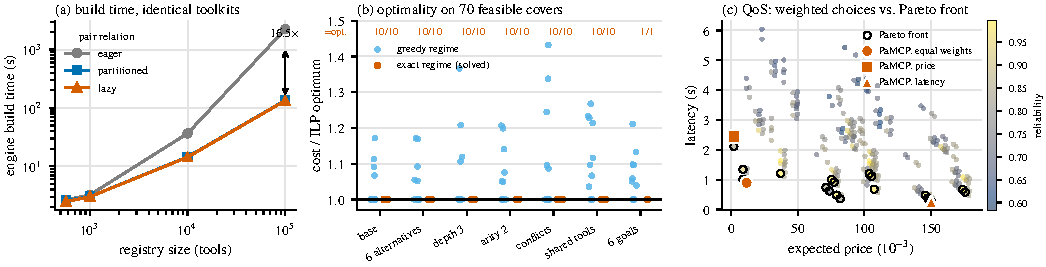
\includegraphics[width=\textwidth]{fig_tsc_eff}
\caption{RQ3/RQ4. (a) Engine build time by pair-relation mode (identical toolkits on all test tasks). (b) Cost of the
greedy and the exact regime relative to the ILP optimum (top: exact equals optimum / solved). (c) The 256 toolkits
of a QoS instance, their Pareto front and \pamcp{}'s choices under three weightings.}
\label{fig:ev-eff}
\end{figure*}

\emph{Results.} On the real registry a request takes 49\,ms at the median (eligibility 0.08\,ms; RAG-MCP's single
dense ranking 12\,ms) and 2.7\,s at $10^5$ cloned tools. Deciding the pairwise risk relation lazily or by effect
class gives identical toolkits on all test tasks and builds the engine at $10^5$ tools in 133--134\,s instead of
2,224\,s, 16.5 times faster with near-linear growth (Fig.~\ref{fig:ev-eff}a); on heterogeneous registries of
$10^4$ tools the lazy build takes 4.6--5.9\,s. Wherever the exact search finishes it returns the ILP optimum (61 of
61 solved instances across alternatives, depth, arity, conflicts and shared tools), it recognises all ten
infeasible instances, and the greedy regime is 4.4--12.6\% above the optimum on average (Fig.~\ref{fig:ev-eff}b);
with six goals the search exhausts its budget and falls back to greedy (6.9\% above). When providers differ in
price, latency and reliability, every equal-weight choice is Pareto-optimal and meets the utility floor, and
weights move the choice along the front as intended (price only: 0.33$\times$ price; latency only: 0.73$\times$
latency; Fig.~\ref{fig:ev-eff}c). Under change, an incremental update takes 13.5\,ms against 4.2\,s for a rebuild,
the exact invalidation of Proposition~3 touches 1.1\% of the cached toolkits instead of all, and all 20 simulated
rug pulls lose their evidence. Experience reuse serves 32.7\% of 300 requests without an analyst call, with
unchanged certification (82.7\% against 82.3\%) and no violation in 89 revalidation probes (removed servers,
revoked or rewritten tools, stricter principal, other model). Deterministic repair raises certification from
72.6\% to 87.4\% when counterexamples are induced. \emph{Answer:} the complete engine scales to $10^5$ tools,
composes optimally where it searches exactly, makes Pareto-consistent QoS trade-offs and adapts to change without
losing its guarantees.

\subsection{Summary and Threats to Validity}
\label{sec:ev-threats}

\begin{table}[t]
\centering
\caption{Answers to the research questions. Conf.: confirmatory test ($p_{\mathrm{Holm}}$).}
\label{tab:ev-answers}
\scriptsize
\setlength{\tabcolsep}{2pt}
\begin{tabular}{@{}lp{3.0cm}p{3.15cm}l@{}}
\toprule
RQ & Result & Best baseline & Conf. \\
\midrule
1 & FNR $\le$3.6\% at 83--100\% coverage & self-assessment ECE 0.20--0.39 & -- \\
2 & Exp@5 0\% (swap 2.3--3.9\%), Util $-3.6$ & lexical 9.9\%, MCP default 42.5\% & F4 $<$0.001 \\
2 & labels = execution, 30/30 calls & -- (observed) & -- \\
3 & strict joint 27.7\%, 1.46 tools & 5.3--14.9\%, 0.64--5.2 tools & expl. \\
3 & recall at equal size 0.189 & 0.084--0.200 & F2 n.s. \\
3 & Hit@1 (569) 41.3\% & MCP-Zero 66.7\% & F7 against \\
2/3 & reachable 0/712, definite 0\% & 0.7--8.1\%, 15.8--37.9\% & F5, H5 $<$0.001 \\
4 & build 16.5$\times$ faster; =ILP 61/61 & eager 2,224\,s; greedy +4--13\% & -- \\
4 & update 13.5\,ms; reuse 32.7\% & rebuild 4.2\,s; cold & -- \\
\bottomrule
\end{tabular}
\end{table}

\begin{table}[t]
\centering
\caption{Confirmatory comparisons, fixed before the data they test (F1--F7 before the set-level experiments; H1--H5
in a dated amendment before the revised test runs), Holm-corrected within each family. Differences in points
(tokens for F6), \pamcp{} minus comparator, with 95\% CI.}
\label{tab:ev-family}
\scriptsize
\setlength{\tabcolsep}{2.2pt}
\begin{tabular}{@{}llrlll@{}}
\toprule
 & Comparison & $\Delta$ & 95\% CI & $p_{\mathrm{Holm}}$ & Verdict \\
\midrule
F1 & Group recall vs per-subtask (non-inf., 0.05) & -8.0 & [-16.6, +0.2] & 1.000 & not shown \\
F2 & Size-matched recall vs RAG-MCP & +6.0 & [-1.6, +13.7] & 0.397 & n.s. \\
F3 & Joint feasibility vs per-subtask (elig.) & +4.3 & [-8.5, +18.1] & 1.000 & n.s. \\
F4 & Exp@5 verified vs lexical & -9.9 & [-13.9, -6.6] & $<$0.001 & supports \\
F5 & Reachable attacks vs per-subtask & -2.7 & [-3.9, -1.5] & $<$0.001 & supports \\
F6 & Tokens, full vs NoGap & -16.7 & [-34.6, +1.0] & 0.269 & n.s. \\
F7 & Hit@1 goal contract vs raw RRF (569) & -15.7 & [-21.3, -10.0] & $<$0.001 & against \\
\midrule
H1 & Hit@1 PaMCP-L vs tuned BM25 (569) & +0.3 & [-8.9, +8.8] & 1.000 & n.s. \\
H2 & Hit@1 PaMCP-L vs Eq. (5) (569) & +11.7 & [+3.0, +22.6] & 0.070 & n.s. \\
H3 & Group recall PaMCP-L vs per-subtask (non-inf.) & -8.8 & [-17.6, -0.5] & 1.000 & not shown \\
H4 & Strict joint feas. vs per-subtask (elig.) & +7.4 & [+0.0, +14.9] & 0.277 & n.s. \\
H5 & Definite out-of-scope vs per-subtask & -20.0 & [-28.4, -12.6] & $<$0.001 & supports \\
\bottomrule
\end{tabular}
\end{table}


Table~\ref{tab:ev-answers} summarises the answers and Table~\ref{tab:ev-family} the confirmatory tests. All
confirmatory tests on safety (F4, F5, H5) favour \pamcp{} at $p_{\mathrm{Holm}}<0.001$; the tests on recall and
retrieval do not, and the feasibility advantage under the strict evaluator is exploratory. \emph{Validity.} Effects, types and feasibility are scored against LLM labels;
execution confirms them on 30 calls of six non-adversarial reference servers, and the label swap bounds the effect
of labeller disagreement but not of errors shared by one model family. Reachability is decided offline: whether an
agent follows an injected instruction, and end-to-end task success, require executing the toolkits, which this
study did not do. Baselines are adaptations sharing a TF-IDF and SVD encoder, all tuned on the same development
split; larger registries are cloned or generated and QoS data are synthetic. Executed compositions over isolated
and adversarial servers, human annotation of a stratified tool sample and reproductions of the baselines with their
original encoders are the natural next steps, and the released artifact supports each of them.

\clearpage
\typeout{EVAL-LAST-PAGE: \the\numexpr\value{page}-1\relax}
\IfFileExists{IEEEtran.bst}{\bibliographystyle{IEEEtran}}{\bibliographystyle{unsrt}}
\bibliography{evaluation_final}
\end{document}
